\documentclass[10pt]{article}
\usepackage{fontspec}
\setmainfont{Times New Roman}
\setmonofont[Scale=0.85]{Menlo}
\usepackage[russian]{babel}
\usepackage{amsmath}
\usepackage[a4paper,landscape,margin=1.3cm]{geometry}
\usepackage{graphicx,xcolor,colortbl,array,enumitem}
\arrayrulecolor[HTML]{B5B4AB}\definecolor{head}{HTML}{F0EFEC}
\setlist{nosep,leftmargin=1.3em,itemsep=0.25em}
\setlength{\parindent}{0pt}\setlength{\parskip}{0.45em}
\setlength{\tabcolsep}{3.2pt}\renewcommand{\arraystretch}{1.08}
\definecolor{ink2}{HTML}{52514E}
\begin{document}
\selectlanguage{russian}
{\LARGE\bfseries Головы внимания Qwen3-0.6B: главное, графики и механизм}\\[0.2em]
{\color{ink2} 28 слоёв $\times$ 16 голов $=$ 448 голов. Головы делят ключи и значения: групп 8, по 2 в каждой. Текст для проверки: 8192 токенов теста WikiText-2 (окна по 512 токенов).}

\section*{1. Главное}
\begin{itemize}
\item \textbf{Большинство голов смотрит по расстоянию, а не по смыслу.} Из 448 голов 246 смотрят на заданное расстояние (сам токен, предыдущий, окно), 187 усредняют дальний контекст и только 15 выбирают токены по содержанию.
\item \textbf{Быстрые частоты RoPE кодируют расстояние, медленные~— содержание.} «Предыдущий токен» берёт 0,42 преимущества цели на частотах с периодом меньше 20 токенов. «Тот же токен», индукция и сток берут 0,88, 0,98 и 1,00 на частотах с периодом больше 20 тысяч токенов.
\item \textbf{Самый большой вес нормализации не работает.} В слое 0 вес ключа на компоненте 50 равен 96,5 (медиана 2,3), но запрос на этой компоненте почти нулевой (не больше 0,02) у всех 16 голов. Замена веса на медиану меняет долю внимания дальше 256 токенов с 0,13 до 0,17 в среднем.
\item \textbf{«Предыдущий токен» держится на быстрых частотах на любой глубине.} Таких голов 16 (слои \mbox{0–5}, 7, 9, 15, 20, 23), у 15 из них частоты с периодом меньше 20 токенов дают не меньше четверти преимущества цели.
\item \textbf{Сток создают отдельные нейроны MLP.} 5 нейронов MLP слоя 2 (номера 55, 128, 1489, 321, 46) на позиции 0 срабатывают в 2824–11654 раз сильнее обычного и дают 0,90 записи MLP в этой позиции. Норма остаточного потока там становится в 530 раз больше, чем на других позициях. Сток заметен со слоя 3, приписку «+ сток» имеют 376 голов из 448; в слоях 18–27 на первый токен уходит 0,53–0,78 внимания.
\item \textbf{Индукция собрана из двух голов.} Ключ индукционной головы целиком приходит из предыдущих голов (у 3 из 3 главный источник~— голова «Предыдущий токен»), запрос~— сам текущий токен.
\item \textbf{Чем глубже, тем меньше решает сам токен.} Он объясняет 0,95 запроса в слое 0, 0,60 в слое 5 и 0,41–0,52 после слоя 12.
\item \textbf{Главную частоту запроса питают сначала MLP, потом головы.} В слоях 1–15 до 0,82 главной частоты приходит из MLP предыдущих слоёв, в последних слоях до 0,76~— из голов внимания.
\end{itemize}
\section*{2. Графики}
\noindent\begin{minipage}{\linewidth}
\textbf{Рисунок 1.} Сверху~— куда в среднем уходит внимание голов слоя; снизу~— сколько голов каждого вида в слое.
\begin{center}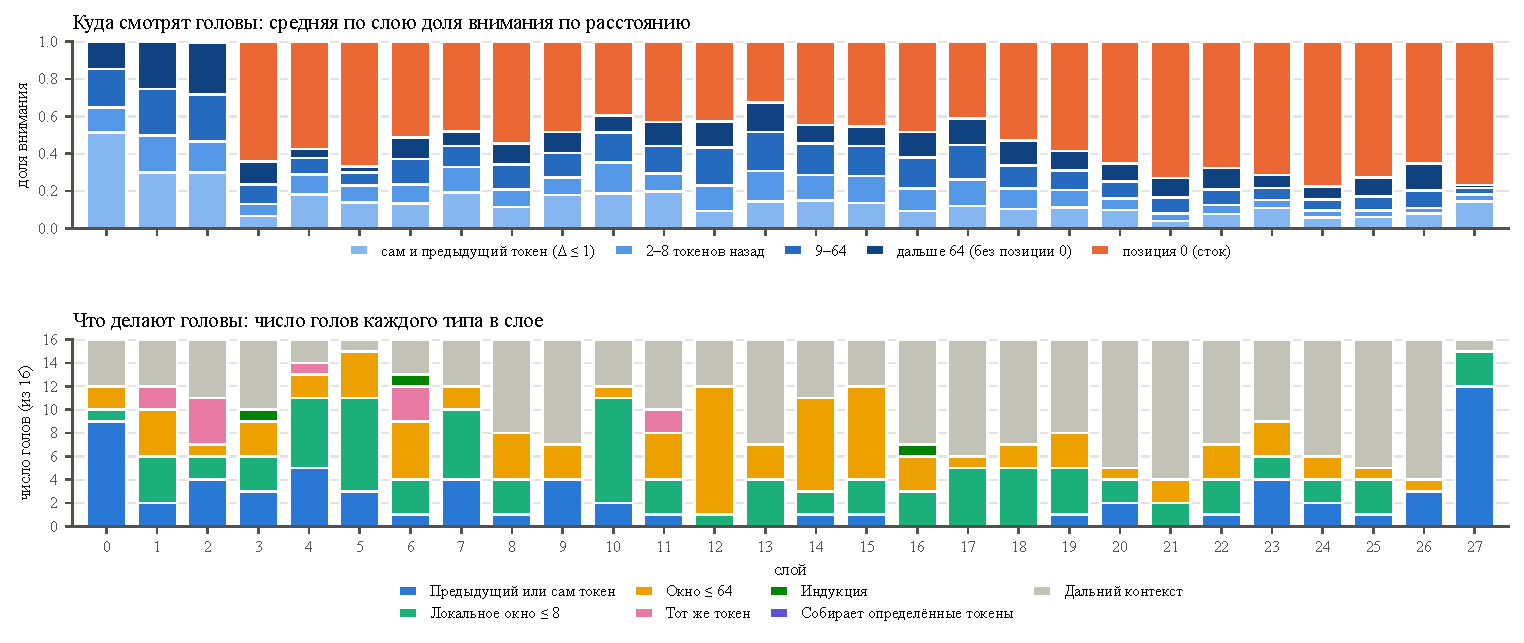
\includegraphics[width=0.76\linewidth]{heads_06b_fig1.pdf}\end{center}
\end{minipage}
\par
\noindent\begin{minipage}{\linewidth}
\textbf{Рисунок 2.} Средние по головам слоя: спад с расстоянием, доля запроса и ключа от токена, источники главной частоты, разброс слагаемых логита, веса нормализации, число ключей.
\begin{center}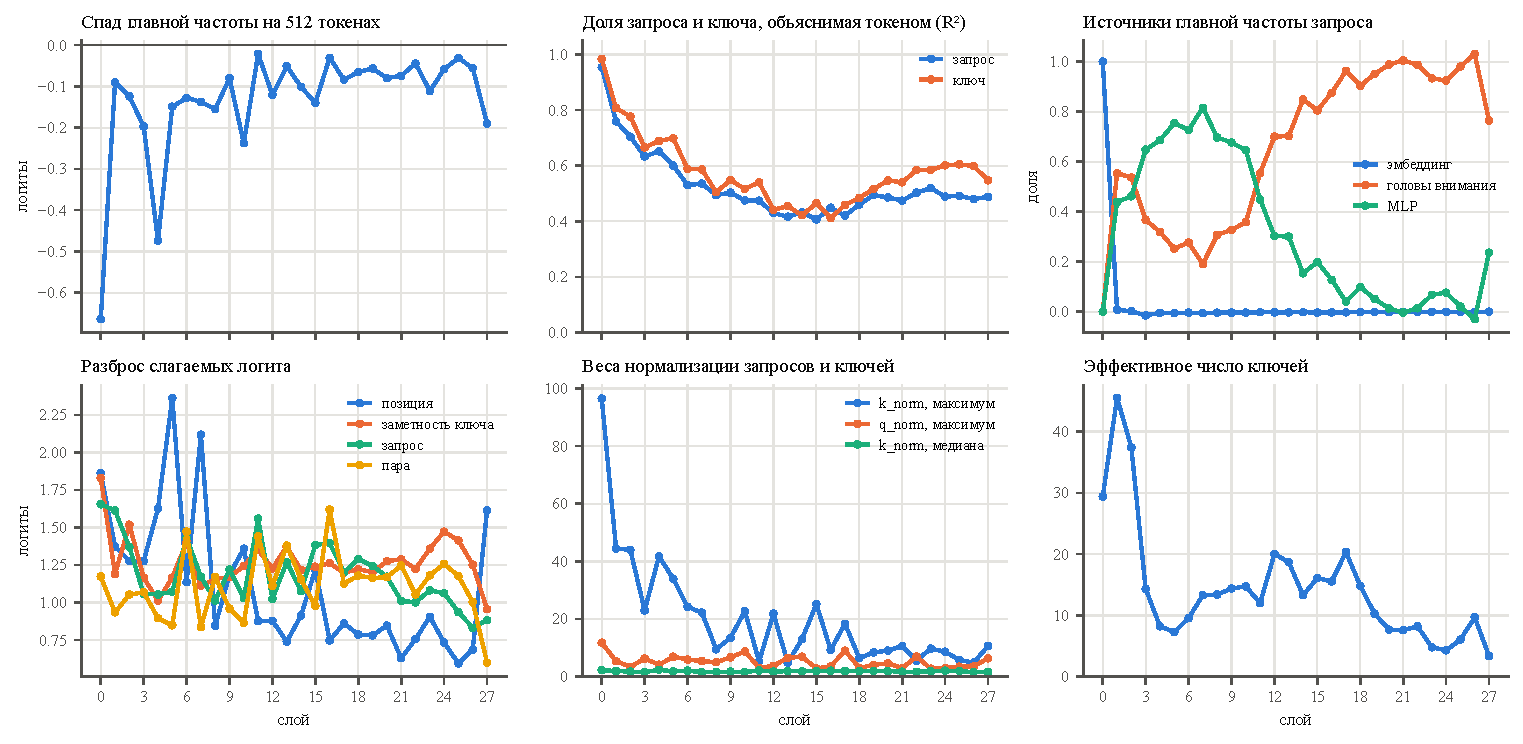
\includegraphics[width=0.78\linewidth]{heads_06b_fig2.pdf}\end{center}
\end{minipage}
\par
\section*{3. Механизм в весах}
\noindent\begin{minipage}{\linewidth}
\textbf{Самый большой вес нормализации не управляет вниманием.} В слое 0 вес k\_norm на компоненте 50 равен 96,5 при медиане 2,3. Это косинусная часть частоты $m{=}50$ с периодом 305971 токенов: на длине контекста она не зависит от расстояния. Значения ключа на этой компоненте большие (сотни), но запрос на ней почти нулевой (не больше 0,02 у всех 16 голов), поэтому в логит компонента почти ничего не даёт. Ниже~— что происходит с головами слоя 0, если этот вес заменить на медиану (запросы с контекстом 1024–2048 токенов): почти ничего.
\begin{center}\begin{tabular}{|l|r|r|r|r|r|r|r|r|r|r|r|r|r|r|r|r|}\hline \rowcolor{head}\textbf{Голова} & \textbf{0} & \textbf{1} & \textbf{2} & \textbf{3} & \textbf{4} & \textbf{5} & \textbf{6} & \textbf{7} & \textbf{8} & \textbf{9} & \textbf{10} & \textbf{11} & \textbf{12} & \textbf{13} & \textbf{14} & \textbf{15} \\ \hline
Дальше 256 токенов, исходные веса & 0,25 & 0,05 & 0,01 & 0,00 & 0,08 & 0,06 & 0,46 & 0,03 & 0,28 & 0,05 & 0,04 & 0,43 & 0,07 & 0,12 & 0,08 & 0,15 \\ \hline
Дальше 256 токенов, вес заменён & 0,30 & 0,07 & 0,01 & 0,00 & 0,13 & 0,09 & 0,53 & 0,04 & 0,33 & 0,06 & 0,05 & 0,45 & 0,14 & 0,21 & 0,10 & 0,18 \\ \hline
Среднее расстояние, исходные веса & 207 & 37 & 14 & 1 & 63 & 42 & 394 & 23 & 241 & 38 & 33 & 367 & 57 & 96 & 58 & 118 \\ \hline
Среднее расстояние, вес заменён & 258 & 51 & 15 & 1 & 100 & 71 & 460 & 29 & 291 & 50 & 41 & 385 & 107 & 163 & 77 & 149 \\ \hline\end{tabular}\end{center}
\end{minipage}
\par
\noindent\begin{minipage}{\linewidth}
\textbf{Какие частоты несут выбор.} Логит~— сумма по частотам RoPE, поэтому преимущество цели точно делится между частотами. Быстрые частоты поворачиваются на длине нескольких токенов и различают расстояние; медленные на длине контекста почти не поворачиваются и сравнивают содержание.
\begin{center}{\small\begin{tabular}{|l|r|r|r|r|r|}\hline
\rowcolor{head}\textbf{Вид головы} & \textbf{Голов} & \textbf{Преим., логиты} & \textbf{Период $<$ 20 токенов} & \textbf{20–20 000} & \textbf{$>$ 20 000 токенов} \\ \hline
Предыдущий токен & 16 & $+$9,5 & 0,42 & 0,56 & 0,02 \\ \hline
Сам токен & 51 & $+$9,2 & 0,22 & 0,60 & 0,19 \\ \hline
Тот же токен & 12 & $+$6,7 & 0,00 & 0,12 & 0,88 \\ \hline
Индукция & 3 & $+$7,2 & 0,00 & 0,02 & 0,98 \\ \hline
Приписка «+ сток» & 376 & $+$9,1 & 0,00 & 0,00 & 1,00 \\ \hline
\hline\end{tabular}}\end{center}
\end{minipage}
\par
\noindent\begin{minipage}{\linewidth}
\textbf{Откуда берётся выбор головы.} Логит линеен и по запросу, и по ключу, а оба точно раскладываются по источникам остаточного потока. Поэтому преимущество цели над остальными токенами (в логитах) делится между источниками без приближений (ошибка суммы 2$\cdot 10^{-5}$ логита).
\begin{center}{\small\begin{tabular}{|l|p{3.7cm}|r|r|c|c|c|p{3.5cm}|}\hline
\rowcolor{head}\textbf{Вид головы} & \textbf{Цель} & \textbf{Голов} & \textbf{Преим., логиты} & \textbf{Ключ: эмб. / головы / MLP} & \textbf{Запрос: эмб. / головы / MLP} & \textbf{Косинус: своя / чужая} & \textbf{Главный источник ключа} \\ \hline
Предыдущий токен & токен перед текущим & 16 & $+$9,5 & 0,07 / 0,47 / 0,46 & 0,07 / 0,49 / 0,44 & 0,05 / 0,05 & MLP3 (7 гол.), MLP0 (3 гол.) \\ \hline
Сам токен & текущий токен & 51 & $+$9,2 & 0,22 / 0,44 / 0,35 & 0,22 / 0,44 / 0,35 & 0,13 / 0,10 & MLP26 (12 гол.), эмб (8 гол.) \\ \hline
Тот же токен & прошлые вхождения того же токена & 12 & $+$6,7 & 0,00 / 0,55 / 0,45 & 0,00 / 0,54 / 0,45 & 0,25 / 0,11 & MLP1 (4 гол.), MLP0 (3 гол.) \\ \hline
Индукция & токен после прошлого вхождения текущего & 3 & $+$7,2 & 0,00 / 1,15 / -0,16 & 0,00 / 0,60 / 0,40 & 0,34 / 0,23 & L2.H12 (1 гол.), L5.H9 (1 гол.) \\ \hline
Приписка «+ сток» & первый токен текста & 376 & $+$9,1 & 0,00 / -0,21 / 1,21 & 0,00 / 0,74 / 0,26 & 0,19 / 0,14 & MLP2 (376 гол.) \\ \hline
\hline\end{tabular}}\end{center}
«Косинус»~— между запросом и ключом одной позиции и разных позиций. У стока доли выходят за пределы 0–1: MLP создают ключ первого токена, а предыдущие головы частично его гасят.
\end{minipage}
\par
\begin{itemize}
\item \textbf{Индукция.} Ключ целиком приходит из предыдущих голов, главным образом из голов «Предыдущий токен» (3.10 ← 2.12 (0,45), 6.11 ← 5.9 (0,29), 16.14 ← 15.3 (0,91)): они записывают в позицию, какой токен стоял перед ней. Запрос несёт сам текущий токен (эмбеддинг / головы / MLP: 0,00 / 0,60 / 0,40). Совпадение даёт цели $+$7,2 логита.
\item \textbf{Сам токен.} У 49 из 51 таких голов пик позиционного ядра приходится на $\Delta{=}0$: быстрые частоты стоят без сдвига и дают 0,22 преимущества цели. Цель получает в среднем $+$9,2 логита. Источники у запроса и ключа одни и те же: в среднем 3,7 из 5 главных совпадают.
\item \textbf{Тот же токен.} Запрос и ключ собраны из одних и тех же источников, которые несут сам токен (эмбеддинг / головы / MLP: 0,00 / 0,54 / 0,45 у запроса и 0,00 / 0,55 / 0,45 у ключа). У одинаковых токенов они совпадают; совпадение идёт по медленным частотам (0,88 преимущества), поэтому не зависит от расстояния. Прошлое вхождение получает $+$6,7 логита.
\item \textbf{Сток.} 5 нейронов MLP слоя 2 (номера 55, 128, 1489, 321, 46) на позиции 0 срабатывают в 2824–11654 раз сильнее обычного и дают 0,90 записи MLP в этой позиции. Норма остаточного потока на позиции 0 вырастает с 1,5 до 529,8 от обычной, 1,00 энергии в координатах 35, 13, 1, 277. Проекция ключей читает этот вектор на медленных частотах (1,00 преимущества): у 376 из 376 голов со стоком главный источник ключа позиции 0~— MLP слоя 2. Постоянный вектор MLP слоя 0, наоборот, пишут многие нейроны: на 90\,\% записи нужно 679 из 3072.
\end{itemize}
\begin{itemize}
\item \textbf{Предыдущий токен.} Быстрые частоты RoPE поворачиваются на заметный угол за один токен (самая быстрая~— на 1 радиан). Фазы запроса и ключа сдвинуты так, что пик приходится на $\Delta{=}1$. Частоты с периодом меньше 20 токенов дают 0,42 преимущества цели.
\end{itemize}
\section*{4. Как получены результаты}
Логит внимания любой головы точно равен сумме по частотам RoPE:
\[ s_h(i,j) \;=\; \frac{1}{\sqrt{D}}\,\mathrm{Re}\sum_{m} z^{q}_{h,m}(i)\,\overline{z^{k}_{g,m}(j)}\,e^{\,i\theta_m (i-j)}, \qquad \theta_m = 10^{-12m/D}, \]
где $z^q$, $z^k$~— запрос и ключ после нормализации (QK-norm), записанные комплексными числами по частотам ($m$-я частота~— компоненты $m$ и $m+D/2$), $\Delta=i-j$~— расстояние между токенами. В слое 0 запрос и ключ зависят только от токена, дальше~— от контекста, поэтому берутся из прогона текста.
\begin{itemize}
\item \textbf{Внимание пересчитано по этой формуле} и совпадает с выходом модели: относительная ошибка не больше $9\cdot 10^{-6}$.
\item \textbf{Источники запроса и ключа найдены точно.} Вход слоя~— сумма эмбеддинга и записей всех предыдущих голов и MLP в остаточный поток. Нормализация и проекции линейны с точностью до одного множителя на позицию, поэтому каждая компонента запроса и ключа раскладывается по источникам без приближений (ошибка суммы не больше $4\cdot 10^{-6}$).
\item \textbf{Позиционное ядро} головы~— логит при средних запросе и ключе как функция расстояния. Оно показывает, как голова смотрит на расстояние независимо от токенов, и раскладывается по частотам: у каждой частоты амплитуда и сдвиг пика.
\end{itemize}
\textbf{Границы отчёта.} Виды голов определены по порогам на одном корпусе (WikiText-2, 8192 токенов). Разложение по источникам объясняет, откуда берутся запрос и ключ, то есть куда голова смотрит; что она после этого записывает в остаточный поток, в отчёт не входит.
\end{document}
